
\section{SIGReg}
\label{appendix:sigreg}
SIGReg proposes to match the distribution of embeddings towards the isotropic Gaussian target distribution. Achieving that match in high-dimension is gracefully done by combining two statistical components (i) Cramer-Wold theorem, and (ii) the univariate Epps-Pulley test-statistic. In short, SIGReg first produces $M$ unit-norm directions $\vu^{(m)}$ and projects the embeddings $\mZ$ onto them as
\begin{align}
    \vh^{(m)}&\triangleq \mZ\vu^{(m)},\vu^{(m)}\in\mathbb{S}^{D-1},\label{eq:h}
\end{align}
where the directions are sampled uniformly on the hypersphere. Then, SIGReg performs univariate distribution matching as
\begin{align}
    {\rm SIGReg}(\mZ)\triangleq \frac{1}{M}\sum_{m=1}^{M}T^{(m)},\tag{SIGReg}\label{eq:SIGreg}
\end{align}
with $T$ the univariate Epps-Pulley test-statistic
\begin{equation}
T^{(m)} = \int_{-\infty}^{\infty} w(t) \left|\phi_N(t; \vh^{(m)}) - \phi_0(t)\right|^2 dt,\tag{EP}\label{eq:EP}
\end{equation}
where the empirical characteristic function (ECF) is defined as $
\phi_N(t; \vh) = \frac{1}{N}\sum_{n=1}^N e^{it \vh_n}$, $w$ is a weighting function, e.g., $w(t) = e^{-\frac{t^2}{2\lambda^2}}$. Lastly, because the target is an isotropic Gaussian in $\mathbb{R}^D$, the univariate projection through $\vu^{(m)}$ makes the univariate target distribution $\phi_0$ the standard Gaussian $N(0,1)$. By Cramér–Wold, matching all 1D marginals implies matching the joint distribution, i.e., in the asymptotic limit over $M$ we have the following weak convergence result
\begin{align}
    {\rm SIGReg}(\mZ)\rightarrow 0 \iff \mathbb{P}_\mZ\rightarrow N(0,\mI).\tag{Cramer-Wold}
\end{align}
Practically, the integral in \eqref{eq:EP} employs a quadrature scheme, e.g., trapezoid with $T$ nodes uniformly distributed in $[0.2,4]$.

\section{Cross-Entropy Method}
\label{appendix:solver}

The \textit{Cross-Entropy Method} (CEM)~\cite{rubinstein2004cross} is a sampling-based (zero-order) optimization algorithm. Intuitively, CEM is an iterative sampling procedure that progressively refines a plan, defined as a sequence of actions, at each iteration.

At every iteration, the algorithm samples a pool of candidate plans from a distribution, 
typically a Gaussian (with initial parameters $\mu=\mathbf{0}$ and $\sigma=\mathbf{I}$). Next, each candidate plan is evaluated using the world model, and a cost is 
associated with it. The algorithm then selects the top $k$ plans with the lowest cost, referred 
to as \textit{elites}. These elites are used to compute statistics that update the parameters of 
the sampling distribution for the next iteration. Through this iterative process, the method 
explores the action space while gradually concentrating the sampling distribution around 
regions associated with lower costs. The final action plan is obtained from the mean of the 
sampling distribution at the last iteration.

However, in non-convex settings, there is no guarantee that the solution to which CEM converges 
is a global optimum. Furthermore, CEM suffers from the curse of dimensionality and becomes 
increasingly difficult to apply when the action space is large.

In our experiments, we use a CEM solver with $300$ sampled action sequences per iteration and 
perform $30$ optimization steps. At each step, the top $30$ candidates are selected as elites 
to update the sampling distribution. We provide the algorithm pseudo-code in Alg.~\ref{alg:cem}.

\setcounter{algorithm}{1}
\begin{algorithm}[h]
\caption{Cross-Entropy Method (CEM) for Action Sequence Optimization}
\label{alg:cem}
\begin{algorithmic}[1]
\Require World model $f$, planning horizon $H$, number of samples $N$, number of elites $K$, number of iterations $T$
\State Initialize sampling distribution parameters $\mu_0 = \mathbf{0}$, $\Sigma_0 = I$
\For{$t = 1$ to $T$}
    \State Sample $N$ candidate action sequences $\{a_{1:H}^{(i)}\}_{i=1}^{N} \sim \mathcal{N}(\mu_{t-1}, \Sigma_{t-1})$
    \For{$i = 1$ to $N$}
        \State Roll out $a_{1:H}^{(i)}$ in the world model $f$
        \State Compute cost $J^{(i)}$
    \EndFor
    \State Select the $K$ sequences with lowest cost (elites)
    \State Update distribution parameters using elite set:
    \State $\mu_t \leftarrow \frac{1}{K}\sum_{i \in \mathcal{E}} a_{1:H}^{(i)}$
    \State $\Sigma_t \leftarrow \text{Var}_{i \in \mathcal{E}}\left(a_{1:H}^{(i)}\right)$
\EndFor
\State \textbf{return} best action sequence found or first action of $\mu_T$
\end{algorithmic}
\end{algorithm}

\section{Baselines} \label{appendix:baselines}

\subsection{DINO-WM}

DINO world model (DINO-WM) focused on learning a predictor by leveraging DINOv2 frozen pre-trained representation to avoid collapse. Because not trained end-to-end, the loss simply is to minimize the predicted next-embedding with the ground trught next-state embedding produced by DINOv2. 

\begin{equation}
    \mathcal{L}_{\text{DINO-WM}} = \frac{1}{BT} \sum_i^B \sum_t^T \| \hat{\vz}^{(i)}_{t+1} - \vz^{(i)}_{t+1} \|_2^2
\end{equation}

We use the same setup as the original paper \citep{zhou2025dino-wm} (architecture, hyper-paremeters, etc..) 

\subsection{PLDM}

PLDM~\citep{sobal2025stresstesting} proposed a method for learning an end-to-end joint-embedding predictive architecture (JEPA). To avoid collapse, their approach takes inspiration from the variance-invariance-covariance regularization (VICReg, \cite{bardes2022vicreg}) with extra terms to take into account the temporality of the next state prediction. The PLDM objective is the following:

\begin{equation}
    \mathcal{L}_{\text{PLDM}} =  \mathcal{L}_{\text{pred}} +  \alpha \mathcal{L}_{\text{var}} +  \beta \mathcal{L}_{\text{cov}} +  \gamma \mathcal{L}_{\text{time-sim}} + \zeta \mathcal{L}_{\text{time-var}} + \nu \mathcal{L}_{\text{time-cov}} + \mu
    \mathcal{L}_{\text{IDM}}
\end{equation}

where,

\begin{equation*}
    \mathcal{L}_{\text{pred}} = \frac{1}{BT} \sum_i^B \sum_t^T \| \hat{\vz}^{(i)}_{t+1} - \vz^{(i)}_{t+1}\|_2^2
\end{equation*}

\begin{equation*}
    \mathcal{L}_{\text{var}} =  \frac{1}{TD} \sum_t^T \sum_d^D \max\left(0,  1-\sqrt{\text{Var}(\vz^{(:)}_{t,d})}+\epsilon\right)
\end{equation*}

\begin{equation*}
    \mathcal{L}_{\text{cov}} =  \frac{1}{T} \sum_t^T \frac{1}{D}\sum_{i\neq j}^D \left[\text{Cov}(\mZ_t)\right]_{ij}
\end{equation*}

\begin{equation*}
    \mathcal{L}_{\text{time-sim}} = \frac{1}{BT} \sum_i^B \sum_t^T \| \vz^{(i)}_t - \vz^{(i)}_{t+1}\|_2^2
\end{equation*}

\begin{equation*}
    \mathcal{L}_{\text{time-var}} =  \frac{1}{BD} \sum_i^B \sum_d^D \max\left(0,  1-\sqrt{\text{Var}(\vz^{(i)}_{:,d})}+\epsilon\right)
\end{equation*}

\begin{equation*}
    \mathcal{L}_{\text{time-cov}} =  \frac{1}{B} \sum_b^B \frac{1}{D}\sum_{i\neq j}^D \left[\text{Cov}(\mZ)\right]_{ij}
\end{equation*}

\begin{equation*}
    \mathcal{L}_{\text{IDM}} = \frac{1}{BT} \sum_i^B \sum_t^T \| \hat{\va}^{(i)}_t - \va^{(i)}_t\|_2^2
\end{equation*}
with $\vz^{(i)}_{t} \in \R^{D}$ correspond to step $t \in [T]$ of trajectory $i \in [B]$ and $T$ is trajectory length and $B$ the batch size, and $\mZ_t \in \mathbb{R}^{B \times D}$ denote the matrix whose $i$-th row is $\vz_t^{(i)}$, i.e.,
\[
\mZ_t =
\begin{bmatrix}
(\vz_t^{(1)})^\top \\
\vdots \\
(\vz_t^{(B)})^\top
\end{bmatrix},
\]
Let $\bar{\mZ}_t$ be the row-centered version of $\mZ_t$:
\[
\bar{\mZ}_t = \mZ_t - \frac{1}{B}\mathbf{1}\mathbf{1}^\top \mZ_t .
\]
Then, for each time step $t$ and feature dimension $d$, the variance across the batch is
\[
\mathrm{Var}(\vz^{(:)}_{t,d})
=
\frac{1}{B-1}\sum_{i=1}^B
\left(
z^{(i)}_{t,d} - \frac{1}{B}\sum_{i'=1}^B z^{(i')}_{t,d}
\right)^2 ,
\]
and the covariance matrix across feature dimensions is
\[
\mathrm{Cov}(\mZ_t)
=
\frac{1}{B-1}\bar{\mZ}_t^\top \bar{\mZ}_t
\in \mathbb{R}^{D \times D}.
\]

Similarly, for the temporal regularization, let $\mZ^{(i)} \in \mathbb{R}^{T \times D}$ denote the matrix whose $t$-th row is $\vz_t^{(i)}$, and let $\bar{\mZ}^{(i)}$ be its row-centered version:
\[
\bar{\mZ}^{(i)} = \mZ^{(i)} - \frac{1}{T}\mathbf{1}\mathbf{1}^\top \mZ^{(i)} .
\]
Then the variance across time is
\[
\mathrm{Var}(\vz^{(i)}_{:,d})
=
\frac{1}{T-1}\sum_{t=1}^T
\left(
z^{(i)}_{t,d} - \frac{1}{T}\sum_{t'=1}^T z^{(i)}_{t',d}
\right)^2 ,
\]
and the temporal covariance matrix is
\[
\mathrm{Cov}(\mZ^{(i)})
=
\frac{1}{T-1}(\bar{\mZ}^{(i)})^\top \bar{\mZ}^{(i)}
\in \mathbb{R}^{D \times D}.
\]

$\hat{\vz}^{(i)}_{t} \in \R^{d}$ is the predicted embedding at step $t$ for traj $i$ using the predictor. $\va^{(i)}_{t} \in \R^{A}$ is the action associated to step $t$ and $\hat{\va}^{(i)}_{t} \in \R^{A}$ is the predicted action for the inverse dynamic model (IDM) $\text{idm}(\vz_t, \vz_{t+1})$.

We select PLDM hyperparameters via a grid search over the loss coefficients. Since the overall objective includes six tunable weights ($\alpha$, $\beta$, $\gamma$, $\zeta$, $\nu$, $\mu$), an exhaustive search over all combinations is not tractable $(\mathcal{O}(n^6))$. Moreover, the original PLDM study reports coefficients that were extensively tuned per environment and dataset, which limits their transferability. We start from the set of hyperparameters from the config provided in their open-source codebase. We motivate this choice by mentioning that no mention of the time-var and time-cov regularization term are mentionned in the original paper. We then perform a grid search for each initial loss coefficient over 256 configurations on Push-T and keep the one performing the best on a held-out set. We report the best hyperparameters found in Table \ref{tab:pldm_init_coeffs}. We kept these coefficients fixed for all training.

\begin{table}[h]
\centering
\begin{tabular}{l c}
\toprule
\textbf{Loss coefficient} & \textbf{Initial value} \\

\toprule
$\alpha$ & 18.0 \\
$\beta$  & 12   \\
$\gamma$ & 0.2  \\
$\zeta$  & 0.7  \\
$\nu$    & 0.0  \\
$\mu$    & 0.0  \\
\bottomrule
\end{tabular}
\vspace{2mm}
\caption{Best coefficient found from grid search.}
\label{tab:pldm_init_coeffs}
\end{table}

\subsection{GC-RL}

To evaluate downstream control, we use goal-conditioned reinforcement learning (GC-RL) with offline training. In particular, we consider goal-conditioned variants of Implicit Q-Learning (IQL) and Implicit Value Learning (IVL). In both cases, observations and goals are encoded using DINOv2 patch embeddings, and policies are trained from offline datasets. Training proceeds in two phases: first learning a value function (and optionally a Q-function), followed by policy extraction via advantage-weighted regression.

\paragraph{GCIQL}
Implicit Q-Learning (IQL) \cite{kostrikov2021offline} is an offline reinforcement learning algorithm that avoids querying out-of-distribution actions by learning a value function via expectile regression. In the goal-conditioned setting, the algorithm learns both a Q-function $Q_\psi(s_t, a_t, g)$ and a value function $V_\theta(s_t, g)$ conditioned on a goal $g$.

The Q-function is trained with Bellman regression, bootstrapping from a target value network $V_{\bar{\theta}}$:

\[
\mathcal{L}_{Q} =
\mathbb{E}_{(s_t, a_t, s_{t+1}, g) \sim \mathcal{D}}
\left[
\left(
Q_\psi(s_t, a_t, g) -
\left(
r(s_t, g) + \gamma m_t V_{\bar{\theta}}(s_{t+1}, g)
\right)
\right)^2
\right],
\]

where $m_t = 0$ if $s_t = g$ (terminal transition) and $m_t = 1$ otherwise.

The value network is trained using expectile regression against targets from the target Q-network $Q_{\bar{\psi}}$:

\[
\mathcal{L}_{V} =
\mathbb{E}_{(s_t, a_t, g) \sim \mathcal{D}}
\left[
L_\tau^2
\left(
Q_{\bar{\psi}}(s_t, a_t, g) - V_\theta(s_t, g)
\right)
\right],
\]

where the expectile loss is defined as

\[
L_\tau^2(u) = |\tau - \mathbbm{1}(u < 0)| u^2 .
\]

The total critic loss is given by

\[
\mathcal{L}_{\text{critic}} = \mathcal{L}_Q + \mathcal{L}_V .
\]

\paragraph{GCIVL}
Implicit Value Learning (IVL) \cite{park2025ogbench} simplifies IQL by removing the Q-function and learning the value function directly through bootstrapped targets. The value network $V_\theta(s_t, g)$ is trained via expectile regression against a target network $V_{\bar{\theta}}$:

\[
\mathcal{L}_{V} =
\mathbb{E}_{(s_t, s_{t+1}, g) \sim \mathcal{D}}
\left[
L_\tau^2
\left(
r(s_t, g) + \gamma V_{\bar{\theta}}(s_{t+1}, g)
-
V_\theta(s_t, g)
\right)
\right].
\]

As in IQL, $L_\tau^2$ denotes the asymmetric expectile loss and $\gamma$ is the discount factor.

\paragraph{Policy extraction.}

For both GCIQL and GCIVL, the policy $\pi_\theta(s_t, g)$ is trained via advantage-weighted regression (AWR). The policy objective is

\[
\mathcal{L}_{\pi} =
\mathbb{E}_{(s_t, a_t, g) \sim \mathcal{D}}
\left[
\exp\left(\beta A(s_t, a_t, g)\right)
\|
\pi_\theta(s_t, g) - a_t
\|_2^2
\right],
\]

where the advantage is computed as

\[
A(s_t, a_t, g) =
r(s_t, g) + \gamma V(s_{t+1}, g) - V(s_t, g),
\]

and $\beta$ is an inverse temperature parameter controlling the strength of advantage weighting.

\subsection{GCBC}

As a simple imitation learning baseline, we consider Goal-Conditioned Behavioral Cloning (GCBC) \cite{ghosh2019learning}. GCBC trains a goal-conditioned policy $\pi_\theta(s_t, g)$ to reproduce expert actions given the current observation $s_t$ and a goal observation $g$. In our implementation, both observations and goals are encoded using DINOv2 patch embeddings before being provided to the policy network.

The policy is trained via supervised learning on an offline dataset $\mathcal{D}$ of state-action-goal tuples. Specifically, the objective minimizes the mean squared error between the predicted action and the action taken in the dataset:

\[
\mathcal{L}_{\text{GCBC}} =
\mathbb{E}_{(s_t, a_t, g) \sim \mathcal{D}}
\left[
\|
\pi_\theta(s_t, g) - a_t
\|_2^2
\right],
\]

where $s_t$ denotes the observation embedding, $g$ the goal embedding, and $a_t$ the corresponding expert action.


\section{Implementation details}
\label{appendix:details}
We apply a frame-skip of 5, grouping consecutive actions between frames into a single action block. This choice enables computationally efficient longer-horizon predictions while maintaining informative temporal transitions. 
We use a batch size of 128 with sub-trajectories of size 4 corresponding to 4 frames and 4 blocks of 5 actions. Each frame is $224\times224$ pixels.  All the training scripts were made with \textbf{stable-pretraining}~\cite{balestriero2025spt}.

\paragraph{Encoder Architecture.}
The encoder is a Vision Transformer Tiny (ViT-Tiny) model from the Hugging Face library, using a patch size of 14.

\paragraph{Predictor Architecture.}
The predictor is implemented as a ViT-S backbone with learned positional embeddings and causal masking over the observation history. The history length is set to 3 for the \textit{PushT} and \textit{OGBench-Cube} environments, and to 1 for \textit{TwoRoom}. During planning, the predictor is used autoregressively to generate rollouts of future latent states.


\paragraph{Decoder (Visualization Only).}
For visualization, we decode the \verb|[CLS]| token embedding (192 dim) from the last encoder layer into an image using a lightweight transformer decoder. The \verb|[CLS]| representation is first projected to a hidden dimension and used as the key and value in cross-attention. A fixed set of learnable query tokens, one for each patch of the target image, interacts with this global representation through several cross-attention layers with residual MLP blocks. For an image of size $224\times224$ with patch size $16$, this corresponds to $P=(224/16)^2=196$ learnable query tokens. The resulting patch embeddings are then linearly projected to $16 \times 16 \times 3$ pixel patches and rearranged to produce a $224 \times 224$ RGB image. This decoder is used only as a diagnostic tool to visualize what visual information is retained in the \verb|[CLS]| representation.

\paragraph{Planning solver.}
For planning, we use the Cross-Entropy Method (CEM). At each planning step, CEM samples 300 candidate action sequences and optimizes them for a maximum of 30 iterations in \textit{PushT} and 10 iterations in the other environments. At each iteration, the top 30 trajectories are retained to update the sampling distribution, and the initial sampling variance is set to 1. The planning horizon is set to 5 steps, which corresponds to 25 environment timesteps due to the use of a frame skip of 5. We employ a receding-horizon Model Predictive Control (MPC) scheme with a horizon of 5, meaning that the entire optimized action sequence is executed before replanning. This configuration follows the setup used in \cite{zhou2025dino-wm}.

\paragraph{Implementation and hardware.}
All experiments are implemented using the \href{https://github.com/rbalestr-lab/stable-worldmodel}{\texttt{stable-worldmodel}}~\cite{maes_lelidec2026swm} framework. Training relies on the \href{https://github.com/rbalestr-lab/stable-pretraining}{\texttt{stable-pretraining}}~\cite{balestriero2025spt} library, while evaluation is performed using PyTorch~\cite{paszke2019torch} and Gymnasium~\cite{towers2024gymnasium}. Both training and planning were performed on a single NVIDIA L40S GPU.

\section{Environment \& Dataset} \label{appendix:envs}

\begin{enumerate}[a)]

\item \textbf{TwoRoom} is a simple continuous 2D navigation task introduced by \citet{sobal2025stresstesting}. The environment consists of two rooms separated by a wall with a single door connecting them. The agent (represented as a red dot) must navigate from a random starting position in one room to a randomly sampled target location in the other room, which requires passing through the door. We collect 10,000 episodes with an average trajectory length of 92 steps. The data are generated using a simple noisy heuristic policy that first directs the agent toward the door along a straight-line path and then toward the target location once the agent has crossed into the other room. Each world model is trained on this dataset for 10 epochs.

\item \textbf{PushT} is a continuous 2D manipulation task in which an agent (represented as a blue dot) must push a T-shaped block to match a target configuration, with interactions restricted to pushing actions. We follow the same setup and dataset as \citet{zhou2025dino-wm}, which contains 20,000 expert episodes with an average length of 196 steps. However, we train each world model for only 10 epochs. Empirically, we observe that 10 epochs are sufficient to reach the best performance, matching the results reported in the DINO-WM paper.

\item \textbf{OGBench-Cube} is a continuous 3D robotic manipulation task in which a robotic arm with an end-effector must pick up a cube and place it at a target location. Originally introduced by \citet{park2025ogbench}, we consider only the single-cube variant. We collect 10,000 episodes, each consisting of 200 steps. The data are generated using the data-collection heuristic provided in the benchmark library. Each world model is trained on this dataset for 10 epochs.

\item \textbf{Reacher} is a continuous control environment from the DeepMind Control Suite~\cite{tassa2018deepmind}. The task consists of controlling a two-joint robotic arm to reach a target location in a 2D plane. Following the setup used in DINO-WM, we consider the variant where success is defined by the perfect alignment of the arm joints with the target configuration required to reach the goal position. We train each world model for 10 epochs on a dataset of 10,000 episodes, each with 200 steps. The data are collected using a Soft Actor-Critic policy.

\end{enumerate}

\section{Evaluation Details}

\begin{figure}[t]
    \centering
    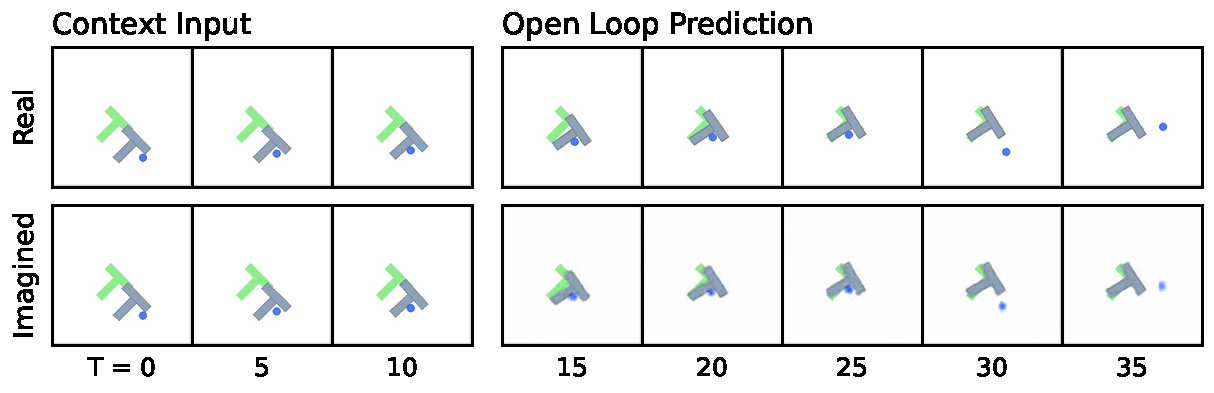
\includegraphics[width=\linewidth]{figs/pusht_rollout_2.pdf}\\
    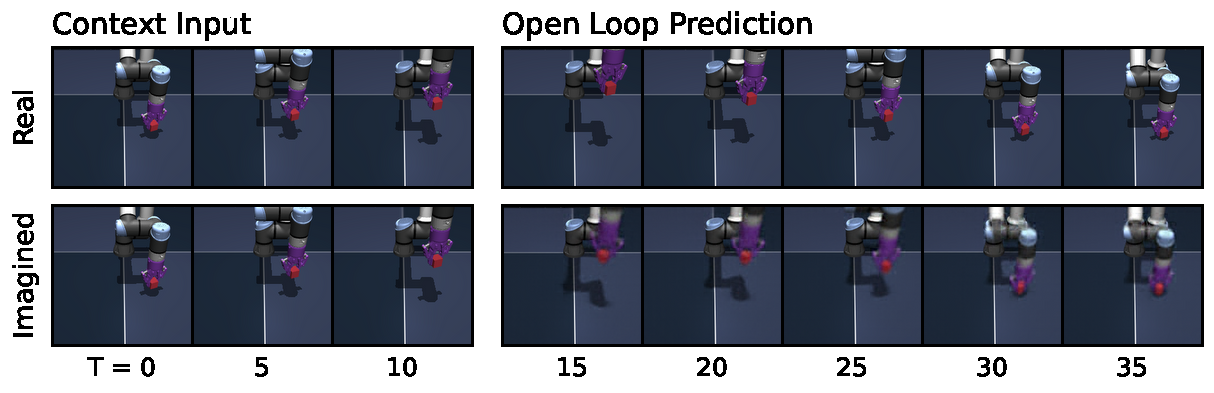
\includegraphics[width=\linewidth]{figs/cube_rollout_2.pdf}
    \caption{\small \textbf{Additional predictor rollouts on PushT (top) and OGBench-Cube (bottom).} Same setup as Fig.~\ref{fig:rollout}: three context frames are encoded into latent representations, and the predictor autoregressively generates future latent states conditioned on the action sequence. All predictions are decoded using a decoder not used during training. On PushT, the imagined trajectory closely tracks the real one, accurately capturing both agent and block motion. On OGBench-Cube, the model preserves the overall scene layout and cube displacement but loses finer details such as end-effector orientation at longer horizons, consistent with the lower probing accuracy on rotational quantities reported in Tab.~\ref{tab:probe-cube}.}
    \label{fig:rollout-2}
\end{figure}

\subsection{Control} \label{appendix:control_details}

We evaluate LeWM on goal-conditioned control tasks in the three environments introduced previously. Control performance is measured using two parameters: the evaluation budget and the distance to the goal. The evaluation budget corresponds to the maximum number of actions the agent is allowed to execute in the environment. The goal distance determines how far in the future the goal state is sampled relative to the initial state.
During evaluation, trajectories are sampled from the offline dataset. The initial state is chosen by randomly sampling a state from a trajectory in the dataset, while the goal state corresponds to a state occurring several timesteps later in the same trajectory. This ensures that the goal is reachable and consistent with the dataset dynamics.
In \textit{TwoRoom}, the evaluation budget is set to 150 steps and the goal state is sampled 100 timesteps in the future. In \textit{PushT}, the evaluation budget is 50 steps and the goal is sampled 25 timesteps in the future. In \textit{OGBench-Cube} and \textit{Reacher}, the evaluation budget is 50 steps, and the goal is sampled 25 timesteps in the future.


\subsection{Probing} \label{appendix:probing}

We use probing to analyze the information contained in the learned latent representations across the three environments. Specifically, we train both linear and non-linear probes to predict physical quantities from the latent embeddings. Linear probes evaluate whether the information is linearly accessible in the latent space, while non-linear probes assess whether the information is present but potentially entangled.

For each probe, we report the mean squared error (MSE) and the Pearson correlation coefficient between the predicted and ground-truth quantities.

The probed variables differ across environments. In \textit{TwoRoom}, we probe the 2D position of the agent (Tab.~\ref{tab:probe-tworoom}). In \textit{PushT}, we probe both the state of the agent and the state of the block (Tab.~\ref{tab:probe-pusht}). In \textit{OGBench-Cube}, we probe the position of the cube and the position of the robot end-effector (Tab.~\ref{tab:probe-cube}).

\begin{table}[h]
\centering
\caption{\small \textbf{Physical Latent Probing results on TwoRoom.} Although LeWM underperforms PLDM in downstream planning on this environment, it matches or outperforms PLDM across all probing metrics, and both methods substantially outperform DINO-WM on the linear probe. This suggests that the learned latent space captures the underlying physical state equally well and that the planning gap is not due to a less informative representation but rather to other factors such as the dynamics model or the planning procedure itself.}
\begin{tabular}{l c c c c}
\toprule
& \multicolumn{4}{c}{\textbf{Agent Position}}\\
\cmidrule(lr){2-5}
& \multicolumn{2}{c}{Linear} & \multicolumn{2}{c}{MLP}\\
\cmidrule(lr){2-3} \cmidrule(lr){4-5}
\textbf{Model} & MSE $\downarrow$ & r $\uparrow$ & MSE $\downarrow$ & r $\uparrow$\\
\toprule
DINO-WM & $0.488 \pm 0.451$ & $0.824$ & $0.000 \pm 0.000$ & $0.999$\\
PLDM & $0.008 \pm 0.041$ & $0.996$ & $0.000 \pm 0.000$ & $1.000$\\
\midrule
LeWM & $0.008 \pm 0.018$ & $0.996$ & $0.000 \pm 0.000$ & $1.000$\\ 
\bottomrule
\end{tabular}
\vspace{2mm}
\label{tab:probe-tworoom}
\end{table}

\begin{table}[h]
\centering
\caption{\small \textbf{Physical latent probing results on OGBench-Cube.} LeWM matches or outperforms PLDM on most properties and achieves the best results on positional quantities such as block position and end-effector position. DINO-WM retains a clear advantage on dynamic and rotational properties (joint velocity, end-effector yaw), likely because such quantities benefit from the richer visual priors learned during large-scale pretraining. All three methods struggle to recover block orientation (quaternion and yaw), suggesting that fine-grained rotational information remains difficult to encode in compact latent spaces
regardless of the training strategy.}
\resizebox{\textwidth}{!}{%
\begin{tabular}{l l c c c c}
\toprule
& & \multicolumn{2}{c}{\textbf{Linear}} & \multicolumn{2}{c}{\textbf{MLP}}\\
\cmidrule(lr){3-4} \cmidrule(lr){5-6}
\textbf{Property} & \textbf{Model} & MSE $\downarrow$ & r $\uparrow$ & MSE $\downarrow$ & r $\uparrow$\\
\toprule
\multirow{3}{*}{Joint Position}
  & DINO-WM & $0.960 \pm 1.150$ & $0.808$ & $0.200 \pm 0.967$ & $0.870$\\
  & PLDM    & $0.372 \pm 1.172$ & $0.695$ & $0.340 \pm 1.164$ & $0.728$\\
  & LeWM    & $0.352 \pm 1.173$ & $0.706$ & $0.330 \pm 1.157$ & $0.742$\\
\midrule
\multirow{3}{*}{Joint Velocity}
  & DINO-WM & $0.792 \pm 0.748$ & $0.763$ & $0.263 \pm 0.683$ & $0.852$\\
  & PLDM    & $1.016 \pm 0.905$ & $0.115$ & $0.661 \pm 0.830$ & $0.536$\\
  & LeWM    & $1.021 \pm 0.902$ & $0.095$ & $0.818 \pm 0.899$ & $0.386$\\
\midrule
\multirow{3}{*}{End-Effector Position}
  & DINO-WM & $0.024 \pm 0.010$ & $0.996$ & $0.004 \pm 0.003$ & $0.999$\\
  & PLDM    & $0.052 \pm 0.073$ & $0.974$ & $0.013 \pm 0.029$ & $0.993$\\
  & LeWM    & $0.018 \pm 0.025$ & $0.991$ & $0.003 \pm 0.004$ & $0.998$\\
\midrule
\multirow{3}{*}{End-Effector Yaw}
  & DINO-WM & $3.317 \pm 1.016$ & $0.828$ & $0.167 \pm 0.168$ & $0.917$\\
  & PLDM    & $0.996 \pm 0.165$ & $0.056$ & $0.985 \pm 0.207$ & $0.117$\\
  & LeWM    & $0.980 \pm 0.295$ & $0.124$ & $0.952 \pm 0.369$ & $0.213$\\
\midrule
\multirow{3}{*}{Gripper}
  & DINO-WM & $0.114 \pm 0.095$ & $0.943$ & $0.038 \pm 0.060$ & $0.982$\\
  & PLDM    & $0.234 \pm 0.169$ & $0.876$ & $0.066 \pm 0.111$ & $0.967$\\
  & LeWM    & $0.121 \pm 0.111$ & $0.938$ & $0.048 \pm 0.079$ & $0.976$\\
\midrule
\multirow{3}{*}{Block Position}
  & DINO-WM & $0.085 \pm 0.029$ & $0.991$ & $0.007 \pm 0.007$ & $0.998$\\
  & PLDM    & $0.031 \pm 0.023$ & $0.985$ & $0.003 \pm 0.004$ & $0.999$\\
  & LeWM    & $0.007 \pm 0.010$ & $0.997$ & $0.002 \pm 0.003$ & $0.999$\\
\midrule
\multirow{3}{*}{Block Quaternion}
  & DINO-WM & $1.596 \pm 10.457$ & $0.257$ & $0.769 \pm 8.046$ & $0.411$\\
  & PLDM    & $1.021 \pm 12.600$ & $0.066$ & $0.989 \pm 12.140$ & $0.218$\\
  & LeWM    & $1.019 \pm 12.596$ & $0.087$ & $0.963 \pm 11.450$ & $0.224$\\
\midrule
\multirow{3}{*}{Block Yaw}
  & DINO-WM & $4.223 \pm 2.530$ & $0.176$ & $0.916 \pm 0.278$ & $0.304$\\
  & PLDM    & $0.996 \pm 0.088$ & $0.061$ & $0.989 \pm 0.140$ & $0.106$\\
  & LeWM    & $0.996 \pm 0.094$ & $0.062$ & $0.973 \pm 0.199$ & $0.164$\\
\midrule
\multirow{3}{*}{\textbf{Overall}}
  & DINO-WM & $1.162 \pm 1.579$ & $0.725$ & $0.290 \pm 1.202$ & $0.799$\\
  & PLDM    & $0.611 \pm 1.875$ & $0.464$ & $0.503 \pm 1.809$ & $0.600$\\
  & LeWM    & $0.592 \pm 1.874$ & $0.477$ & $0.525 \pm 1.714$ & $0.584$\\
\bottomrule
\end{tabular}%
}
\label{tab:probe-cube}
\end{table}

\subsection{Violation-of-expectation}\label{appendix:voe}

We evaluate physical understanding using the violation-of-expectation (VoE) framework across three environments. In each environment, we generate three types of trajectories: an unperturbed reference trajectory, a trajectory containing a visual perturbation, and a trajectory containing a physical perturbation. Visual perturbations correspond to abrupt color changes of an object, while physical perturbations correspond to teleporting objects to random positions, thereby violating physical continuity. Examples of trajectories are shown in Figure~\ref{fig:voe_frames}.

\paragraph{TwoRoom.}
In the \textit{TwoRoom} environment, the agent is controlled by an expert policy that navigates toward a goal position. We generate three trajectories: (1) an unperturbed trajectory, (2) a trajectory where the color of the agent changes midway through the episode, and (3) a trajectory where the agent is teleported to a random position at the same timestep. The resulting surprise signals for PLDM and DINO-WM are shown in the left panels of Figures~\ref{fig:voe_surprise_pldm} and~\ref{fig:voe_surprise_dinowm}, respectively.

\paragraph{PushT.}
In the \textit{PushT} environment, the agent is controlled by a random policy biased toward interacting with the block. As before, we construct three trajectories: (1) an unperturbed trajectory, (2) a trajectory where the color of the block changes abruptly during the episode, and (3) a trajectory where both the agent and the block are teleported to random positions at the perturbation timestep. The corresponding surprise signals for PLDM and DINO-WM are shown in the center panels of Figures~\ref{fig:voe_surprise_pldm} and~\ref{fig:voe_surprise_dinowm}.

\paragraph{OGBench-Cube.}
In the \textit{OGBench-Cube} environment, the agent follows an expert policy that picks up the cube and places it at a target position. We again consider three trajectories: (1) an unperturbed trajectory, (2) a trajectory where the cube's color changes during the episode, and (3) a trajectory where the cube is teleported to a random position midway through the trajectory. The resulting surprise signals for PLDM and DINO-WM are shown in the right panels of Figures~\ref{fig:voe_surprise_pldm} and~\ref{fig:voe_surprise_dinowm}.

\begin{figure}
    \centering
    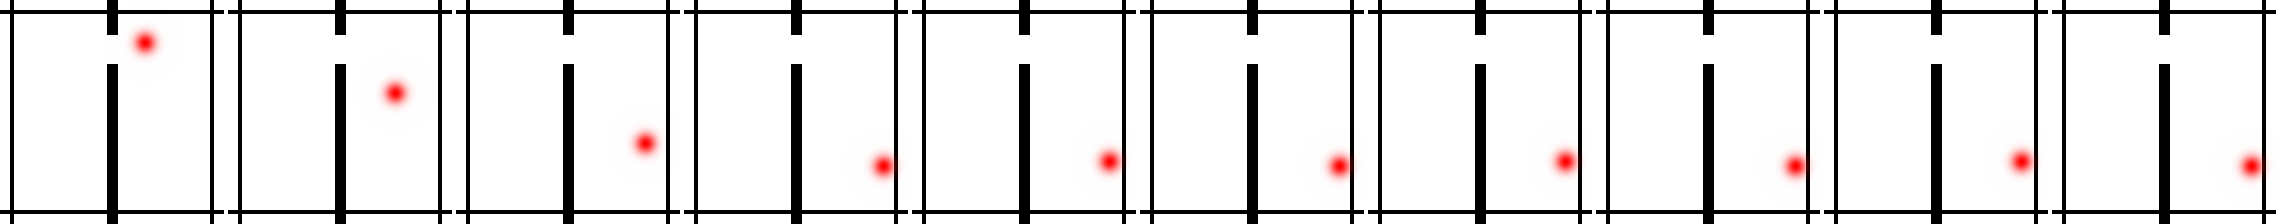
\includegraphics[width=\linewidth]{figs/strip_tworoom_control_1.png}
    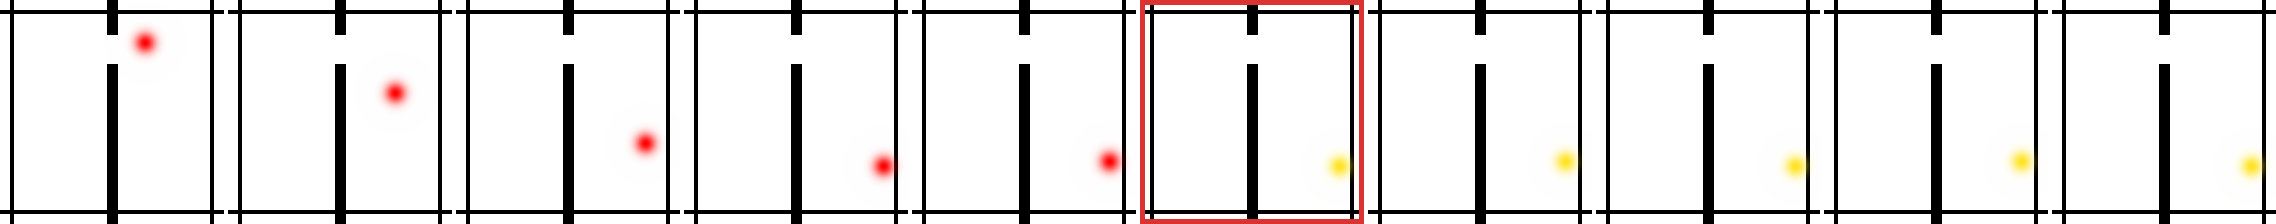
\includegraphics[width=\linewidth]{figs/strip_tworoom_agent_color_1.png}
    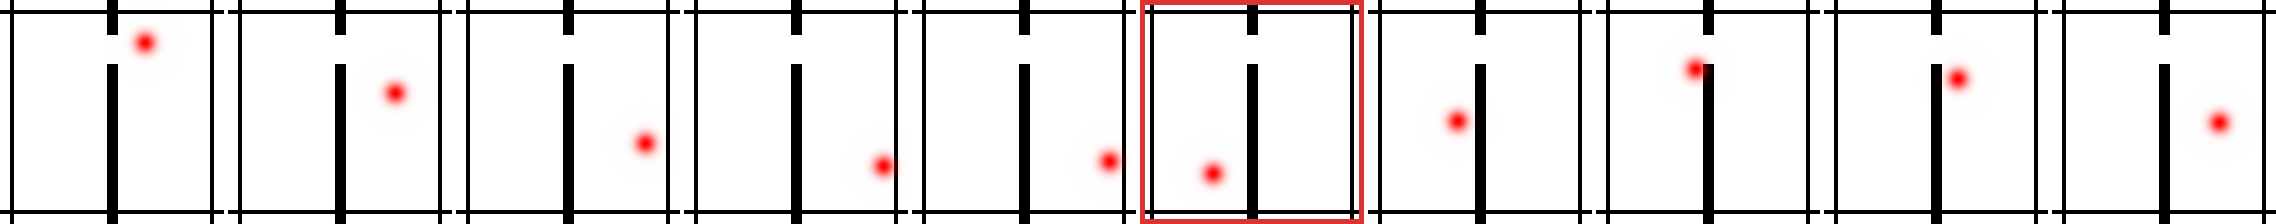
\includegraphics[width=\linewidth]{figs/strip_tworoom_teleport_1.png}
    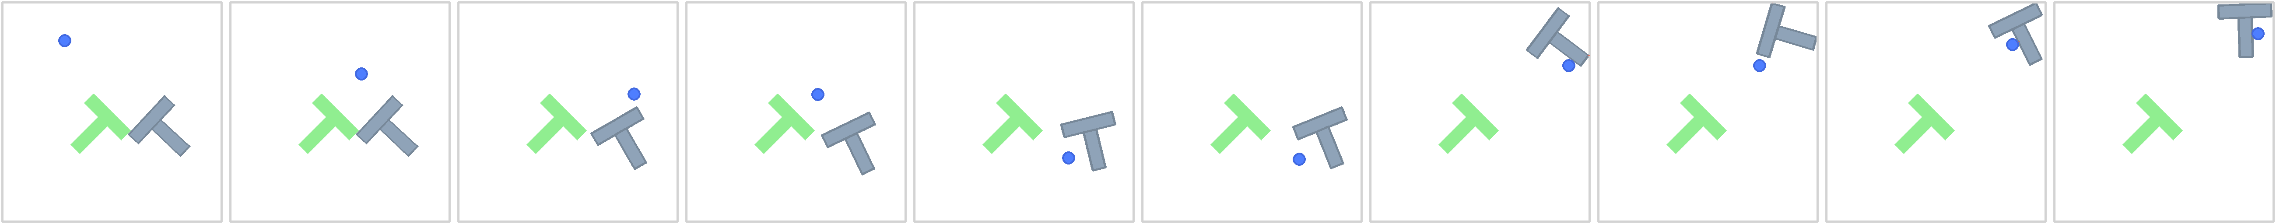
\includegraphics[width=\linewidth]{figs/strip_pusht_control_4.png}
    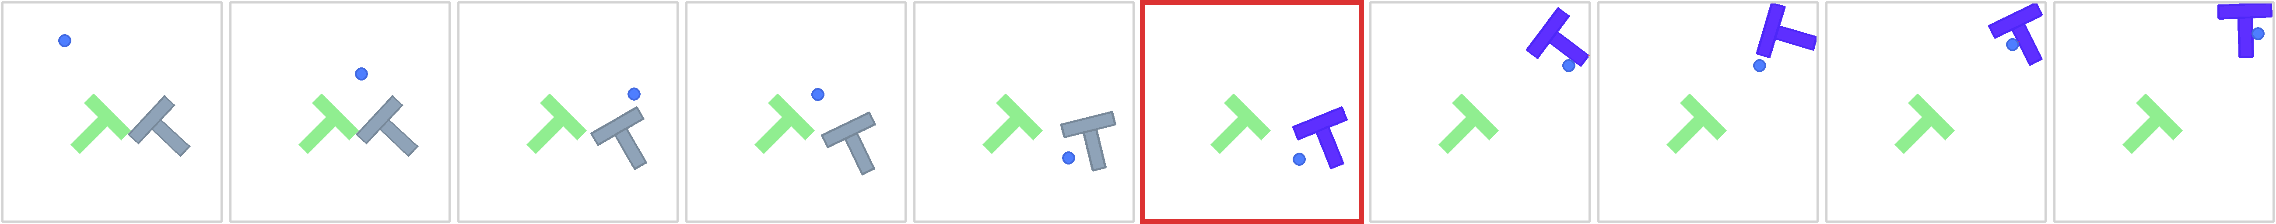
\includegraphics[width=\linewidth]{figs/strip_pusht_block_color_4.png}
    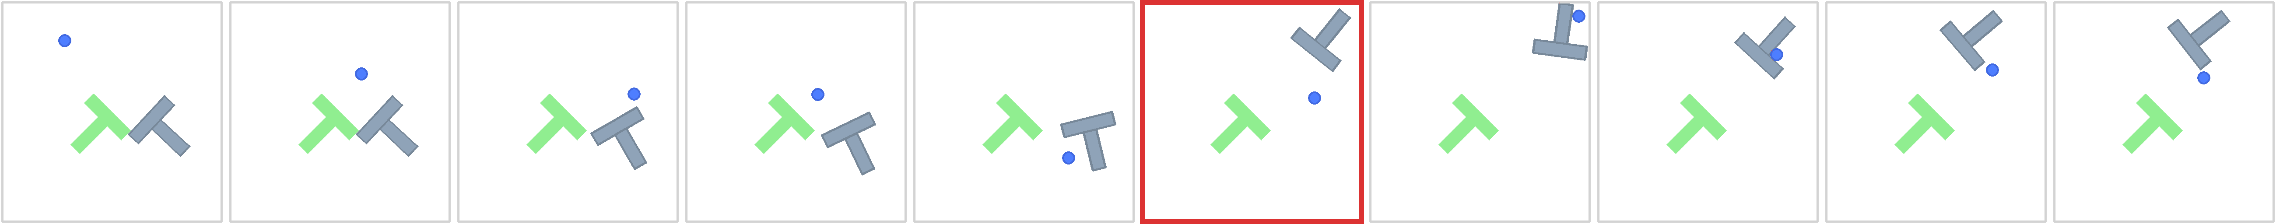
\includegraphics[width=\linewidth]{figs/strip_pusht_teleport_4.png}
    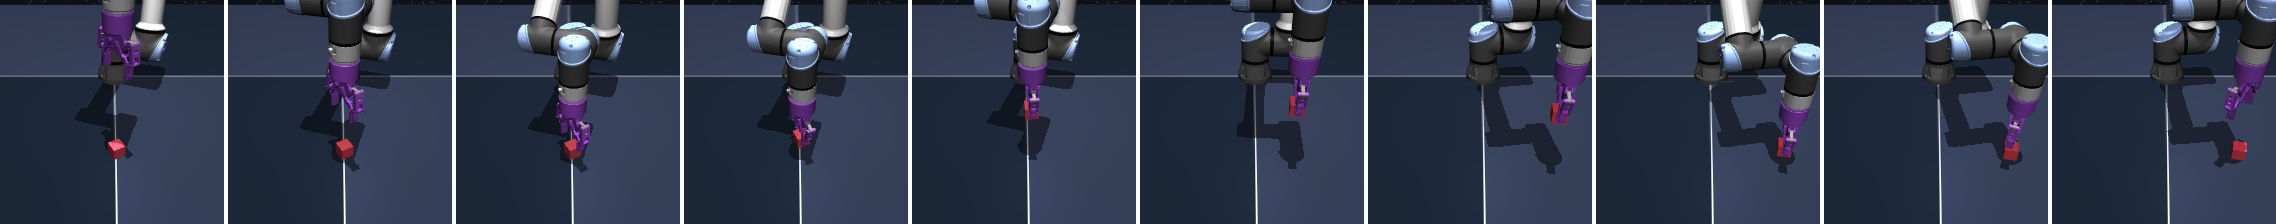
\includegraphics[width=\linewidth]{figs/strip_cube_control_5.png}
    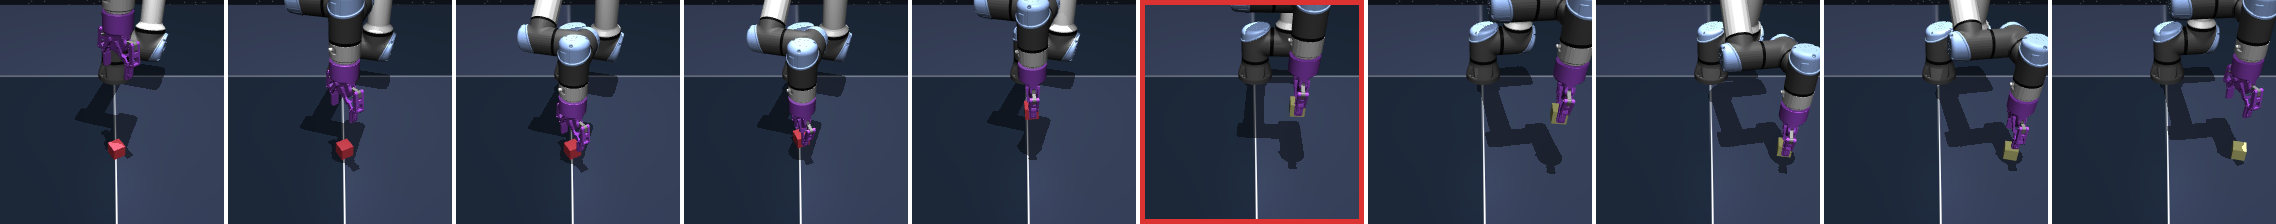
\includegraphics[width=\linewidth]{figs/strip_cube_cube_color_5.png}
    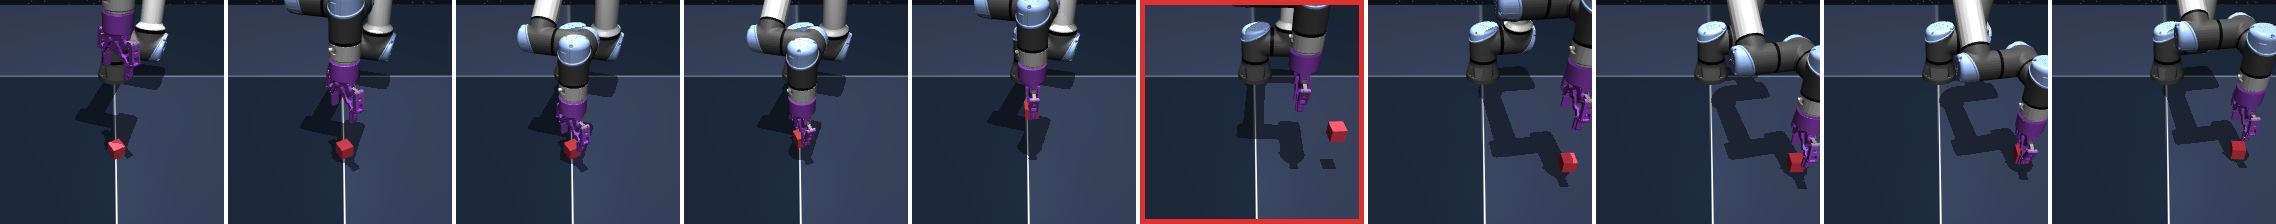
\includegraphics[width=\linewidth]{figs/strip_cube_teleport_5.png}
    \caption{\small \textbf{Example of trajectories used for the Violation of Expectation experiments} (Sec.~\ref{subsec:voe}). For each environment, the first row corresponds to the unperturbed trajectory, the second row corresponds to a trajectory where a visual perturbation occurs and the third row displays trajectories where the state of the system is randomly reset in the middle of the trajectory. The frame where the perturbation occurs is highlighted in red.}
    \label{fig:voe_frames}
\end{figure}

\begin{figure}
    \centering
    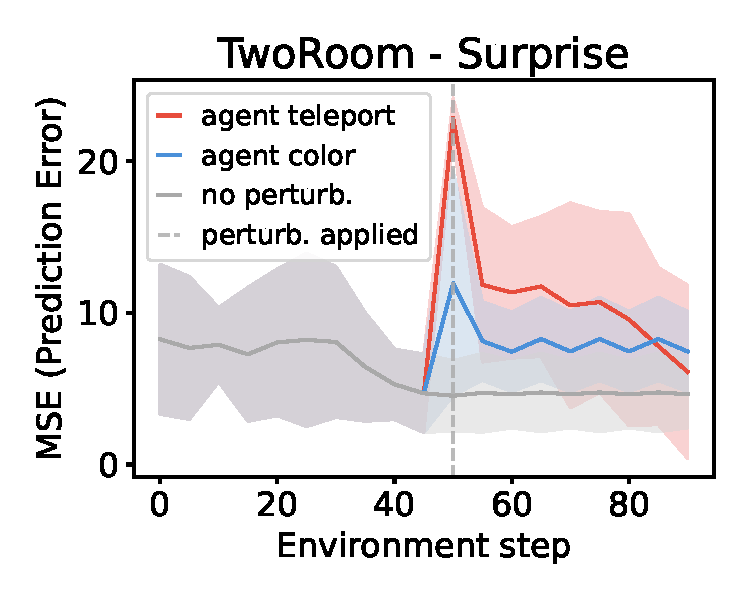
\includegraphics[width=0.32\linewidth]{figs/surprise_tworoom_pldm_epoch_80.pdf}
    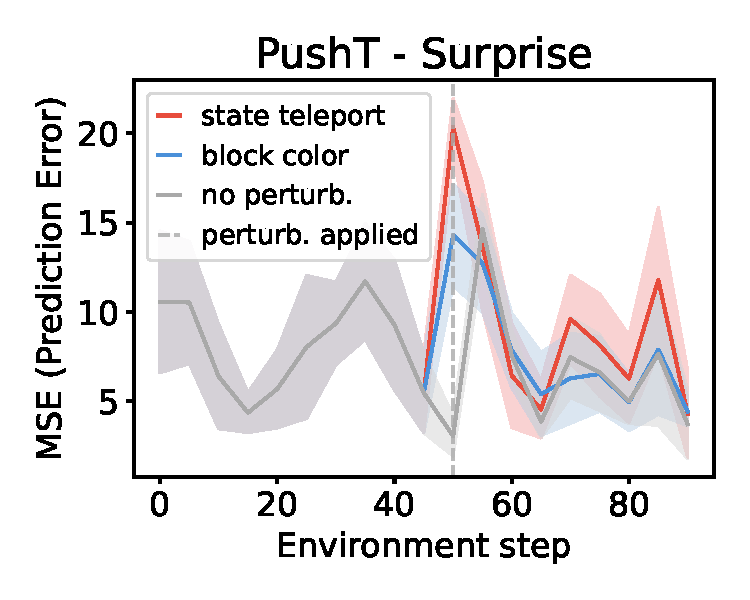
\includegraphics[width=0.32\linewidth]{figs/surprise_pusht_pldm_epoch_10.pdf}
    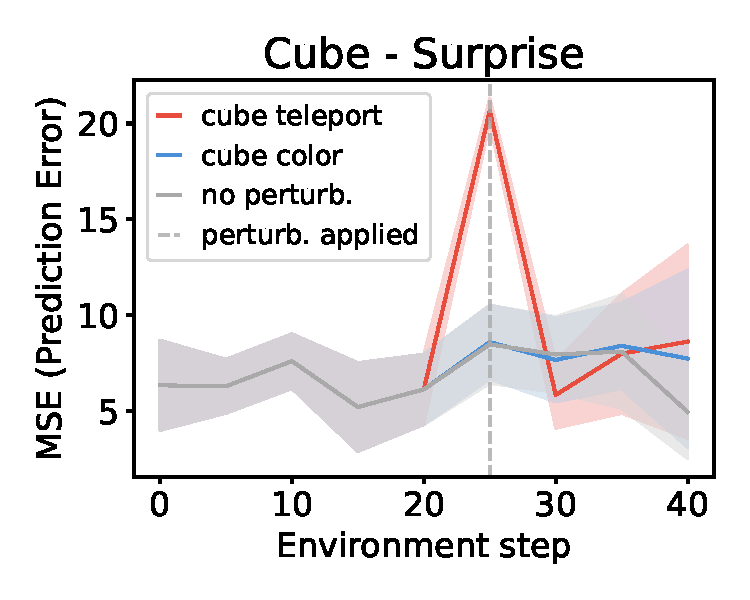
\includegraphics[width=0.32\linewidth]{figs/surprise_cube_pldm_epoch_10.pdf}
    \caption{\textbf{Violation-of-expectation evaluation with PLDM.} From left to right: \textit{TwoRoom}, \textit{PushT}, and \textit{OGBench-Cube}. Surprise is plotted over time for unperturbed, visually perturbed, and physically perturbed trajectories. In \textit{TwoRoom} and \textit{PushT}, the model assigns significantly higher surprise to both visual and physical perturbations. In \textit{OGBench-Cube}, the increase in surprise is weaker and not consistently significant.}
    \label{fig:voe_surprise_pldm}
\end{figure}

\begin{figure}
    \centering
    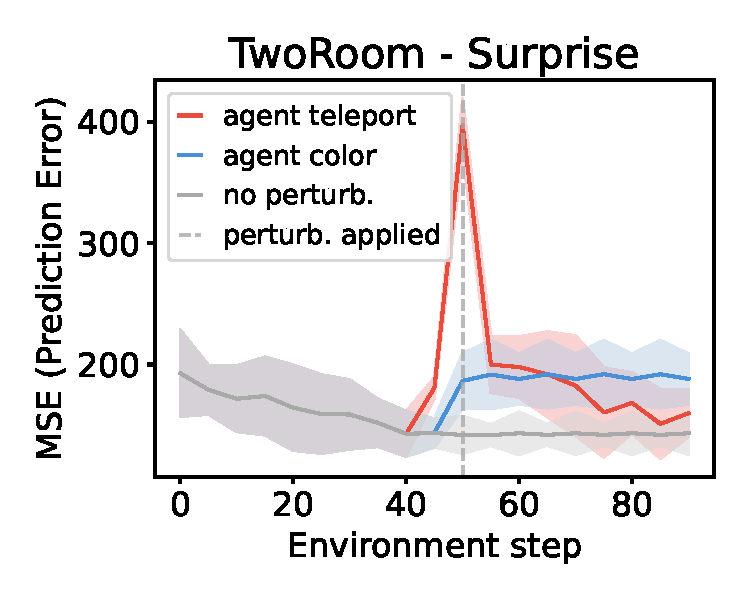
\includegraphics[width=0.3\linewidth]{figs/surprise_tworoom_dinowm_epoch_80.pdf}
    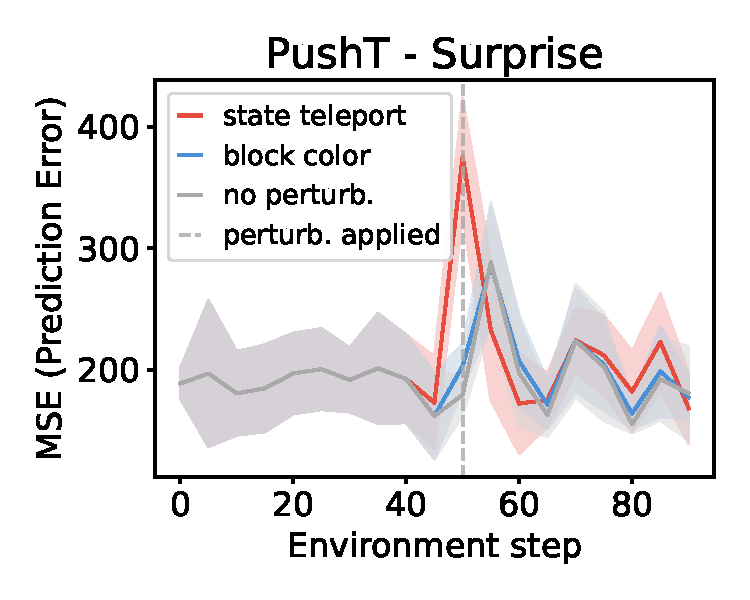
\includegraphics[width=0.3\linewidth]{figs/surprise_pusht_dinowm_epoch_10.pdf}
    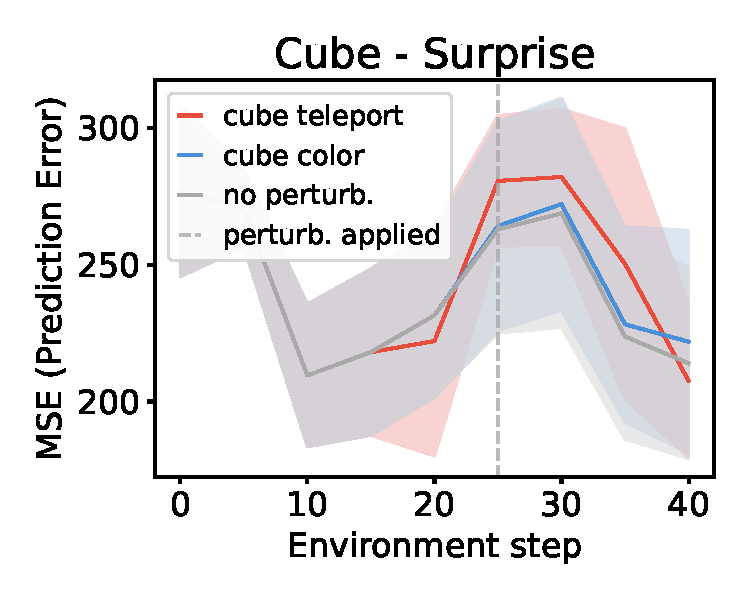
\includegraphics[width=0.3\linewidth]{figs/surprise_cube_dinowm_epoch_10.pdf}
    \caption{\textbf{Violation-of-expectation evaluation with DINO-WM.} From left to right: \textit{TwoRoom}, \textit{PushT}, and \textit{OGBench-Cube}. Surprise is plotted over time for unperturbed, visually perturbed, and physically perturbed trajectories. While the model detects both perturbations in \textit{TwoRoom} and \textit{PushT}, surprise does not increase significantly for either perturbation in \textit{OGBench-Cube}.}
    \label{fig:voe_surprise_dinowm}
\end{figure}



\section{Ablations.}
\label{appendix:ablations}

\begin{figure}[t]
    \centering
    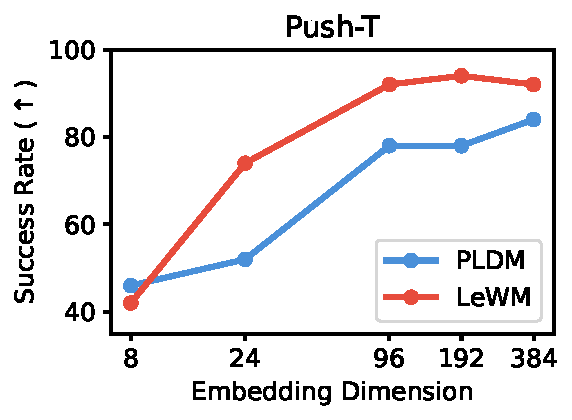
\includegraphics[width=0.32\linewidth]{figs/embed_dim.pdf}
    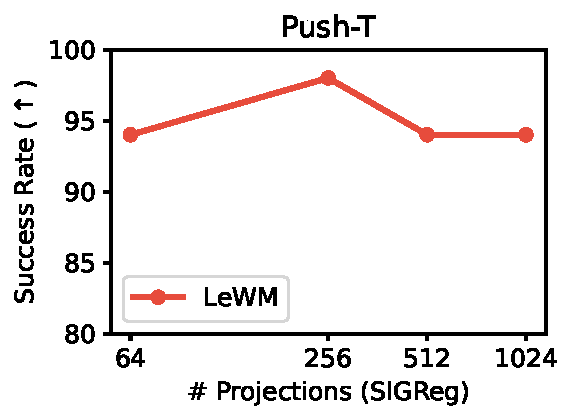
\includegraphics[width=0.32\linewidth]{figs/num_proj.pdf}
    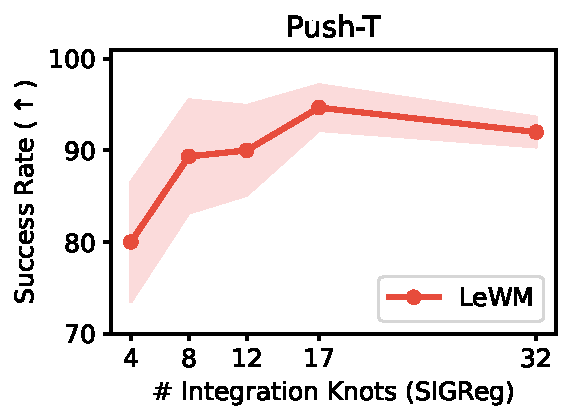
\includegraphics[width=0.32\linewidth]{figs/num_integration.pdf}
    \caption{\textbf{Ablation studies of key design choices in LeWM.} \textbf{Left:} effect of the embedding dimension; performance improves with larger embeddings but quickly saturates beyond a certain threshold. \textbf{Center:} effect of the number of random projections used in SIGReg; performance remains stable, indicating that this parameter is not critical. \textbf{Right:} effect of the number of integration knots used to compute the SIGReg loss; results are similarly insensitive to this parameter.}
    \label{fig:ablation-sigreg}
\end{figure}

\paragraph{Training variance.}
To assess the stability of training, we retrain the model using multiple random seeds. As shown in Tab.~\ref{tab:train-var}, the resulting performance exhibits consistently high success rates with low variance across runs, indicating that the training procedure is stable and reproducible.

\begin{table}[h]
\centering
\caption{\textbf{Training Variance.} We report the mean success rate across three training seeds and the corresponding variance, evaluated over the same set of 50 trajectories on Push-T. The goal configuration is reachable within 25 steps, and we allow a planning budget of 50 steps. PLDM exhibits higher variance compared to DINO-WM and LeWM.}
\begin{tabular}{l c}
\toprule
\textbf{Model} & \textbf{Push-T} (SR $\uparrow$)\\
\toprule
DINO-WM & $92.0 \pm 1.63$\\
PLDM & $78.0 \pm 5.0$ \\
LeWM (ours) & $\bm{96.0} \pm \bm{2.83}$\\
\bottomrule
\end{tabular}
\vspace{2mm}
\label{tab:train-var}
\end{table}

\paragraph{Embedding dimensions.}
We study the impact of the embedding dimensionality on performance. As shown in Fig.~\ref{fig:ablation-sigreg}, performance drops when the embedding dimension falls below a certain threshold (around 184), while increasing the dimension beyond this value yields diminishing returns and leads to performance saturation.


\paragraph{Number of projections in SIGReg.}
We study the impact of the number of projections used in SIGReg. As shown in Fig.~\ref{fig:ablation-sigreg}, varying the number of projections has little effect on performance in downstream control tasks. This suggests that the method is largely insensitive to this hyperparameter, and therefore it does not require careful tuning. In practice, this leaves $\lambda$ as the only effective hyperparameter to optimize.

\paragraph{Weight of SIGReg regularization.}
We analyze the effect of the SIGReg regularization weight $\lambda$. As shown in Fig.\ref{fig:abl-lambda}, the method achieves high performance across a wide range of values for $\lambda$. In particular, for $\lambda \in [0.01, 0.2]$, the success rate remains above 80\%. This indicates that the approach is robust to the choice of this parameter. Moreover, since $\lambda$ is the only effective hyperparameter, it can be tuned efficiently, for instance via a simple bisection search.

\begin{figure}
    \centering
    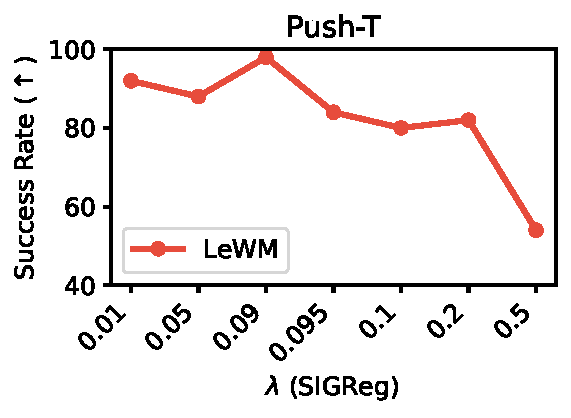
\includegraphics[width=0.5\linewidth]{figs/lambda.pdf}
    \caption{\small \textbf{Effect of the SIGReg regularization weight $\lambda$ on Push-T planning performance.} Success rate remains above 80\% across a wide range of values ($\lambda \in [0.01, 0.2]$), peaking near $\lambda = 0.09$. Performance degrades sharply only at $\lambda = 0.5$, where the regularizer dominates the prediction loss and hinders dynamics modeling. Since $\lambda$ is the only effective hyperparameter of LeWM, the SIGReg loss coefficient is easy to tune via a simple bisection search.}
    \label{fig:abl-lambda}
\end{figure}

\paragraph{Predictor Size.}
We analyze the effect of the predictor size on performance. As shown in Tab.~\ref{tab:pred-size}, the best results are obtained with a ViT-S predictor. Reducing the predictor to a ViT-T model leads to a drop in performance, while increasing the size to ViT-B does not provide additional gains and slightly degrades performance. This suggests that ViT-S offers the best trade-off between model capacity and optimization stability for this task.

\begin{table}
\centering
\caption{\small Effect of the predictor size on planning performance in the Push-T environment. We report the success rate (SR). The ViT-S predictor achieves the best performance.}
\begin{tabular}{l c}
\toprule
\textbf{pred. size} & \textbf{Push-T} (SR $\uparrow$)\\
\toprule
tiny & $80.67 \pm 6.54$\\
small & $\bm{96.0} \pm \bm{2.83}$\\
base & $86.7 \pm 3.06$\\
\bottomrule
\end{tabular}
\label{tab:pred-size}
\end{table}


\paragraph{Decoder.}
We study the impact of adding a reconstruction loss during training. As shown in Tab.~\ref{tab:decoder-loss}, incorporating a decoder and a reconstruction objective does not improve downstream control performance. In fact, performance slightly decreases compared to the model trained without a decoder. This suggests that the JEPA training objective already captures the information necessary for planning, while the reconstruction loss may encourage the model to encode additional visual details that are not relevant for control.


\begin{table}
\centering
\caption{\small Effect of adding a reconstruction loss during training. We report the success rate (SR) on the Push-T planning task. The model trained without the decoder loss achieves higher performance.}
\begin{tabular}{l c}
\toprule
 & \textbf{Push-T} (SR $\uparrow$)\\
\toprule
LeWM w/o decoder loss & $\bm{96.0} \pm \bm{2.83}$\\
LeWM with decoder loss & $86.0 \pm 7.54$\\
\bottomrule
\end{tabular}
\label{tab:decoder-loss}
\end{table}

\paragraph{Architecture.}
We study the impact of encoder architecture on LeWM performance by replacing the ViT encoder with a ResNet-18 backbone. As shown in Tab.~\ref{tab:encoder-arch}, LeWM achieves competitive performance with both architectures, suggesting that it is agnostic to the choice of vision encoder used during training, though ViT retains a modest advantage.

\begin{table}[h]
\centering
\caption{\small \textbf{Encoder Architecture Effect.} We report the success rate (SR) on the Push-T planning task. LeWM achieves competitive performance across encoder architectures, with ViT holding a slight edge.}
\begin{tabular}{l c}
\toprule
 & \textbf{Push-T} (SR $\uparrow$)\\
\midrule
LeWM ViT & $\bm{96.0} \pm \bm{2.83}$\\
LeWM ResNet-18 & $94.0 \pm 3.27$\\
\bottomrule
\end{tabular}
\label{tab:encoder-arch}
\end{table}

\paragraph{Predictor Dropout.}
We analyze the effect of applying dropout in the predictor during training. As shown in Tab.~\ref{tab:pred-drop}, introducing a small amount of dropout significantly improves downstream control performance. In particular, a dropout rate of $0.1$ achieves the highest success rate, while both lower and higher values lead to worse performance. This suggests that moderate dropout helps regularize the predictor and improves generalization, whereas excessive dropout degrades the quality of the learned dynamics.

\begin{table}
\centering
\caption{\small Effect of predictor dropout during training on Push-T planning performance. We report the success rate (SR). A small amount of dropout ($p=0.1$) yields the best results.}
\begin{tabular}{l c}
\toprule
$p$ & \textbf{Push-T} (SR $\uparrow$)\\
\toprule
$0.0$ & $78 \pm 6.54$\\
$0.1$ & $\bm{96.0} \pm \bm{2.83}$\\
$0.2$ & $85.33 \pm 5.74$\\
$0.5$ & $66.67 \pm 4.11$\\
\bottomrule
\end{tabular}
\label{tab:pred-drop}
\end{table}

\section{Temporal Latent Path Straightening.}
\label{appendix:tmp-straight}

The temporal straightening hypothesis, introduced by \citet{henaff2019perceptual}, posits that we represent complex temporal dynamics as smooth, approximately straight trajectories in our representation spaces. This principle has since found applications beyond neuroscience: \citet{interno2025aigenerated} leverage temporal straightness measured from DINOv2 features to discriminate AI-generated videos from real ones, demonstrating that this geometric property carries a meaningful signal about the nature of the underlying dynamics, and \citet{wang2026temporal} shows it can be beneficial for planning.

During training on PushT, we record, for curiosity, the temporal straightness of LeWM's latent trajectories. Given a sequence of latent embeddings $\mathbf{z}_{1:T} \in \mathbb{R}^{B \times T \times D}$, we define the temporal velocity vectors as $\mathbf{v}_t = \mathbf{z}_{t+1} - \mathbf{z}_t$. The path straightening measure is defined as the mean pairwise cosine similarity between consecutive velocities:
\begin{equation}
    \mathcal{S}_{\text{straight}} = \frac{1}{B(T-2)} \sum_{i=1}^{B} \sum_{t=1}^{T-2} \frac{\langle \mathbf{v}_t^{(i)},\, \mathbf{v}_{t+1}^{(i)} \rangle}{\|\mathbf{v}_t^{(i)}\| \, \|\mathbf{v}_{t+1}^{(i)}\|}.
    \label{eq:path-straightening}
\end{equation}
A value of $\mathcal{S}_{\text{straight}}$ close to $1$ indicates that consecutive velocities are nearly collinear, meaning the latent trajectory approaches a straight line. Interestingly, we observe that temporal straightening emerges naturally over the course of training without any training term explicitly encouraging it (Fig.~\ref{fig:tmp-straight}). 

We hypothesize that this emerges because SIGReg is applied independently at each time step but not across the temporal dimension, leaving the temporal structure unconstrained. This allows the encoder to converge toward a form of \emph{temporal collapse}, where successive embeddings evolve along increasingly linear paths. Rather than being detrimental, this implicit bias appears to benefit downstream performance, as shown in Fig.~\ref{fig:ctrl-all}. Notably, LeWM achieves higher temporal straightness than PLDM despite having no explicit regularizer encouraging it, whereas PLDM employs a regularizer on consecutive latent states that directly promotes temporal smoothness.

\begin{figure}
    \centering
    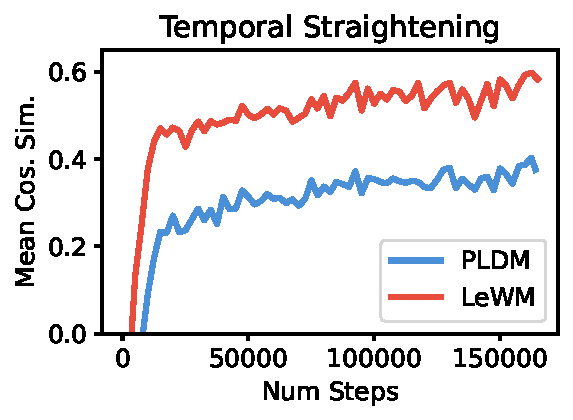
\includegraphics[width=0.5\linewidth]{figs/temporal_straightening.pdf}
    \caption{\textbf{Temporal Latent Straightening on Push-T.} Mean cosine similarity between consecutive latent velocity vectors (Eq.~\ref{eq:path-straightening}) over training. Higher values indicate straighter latent trajectories. PLDM explicitly encourages temporal regularity through a dedicated temporal smoothness loss ($\mathcal{L}_{\text{time-sim}}$), yet LeWM achieves substantially straighter latent paths as a purely emergent phenomenon, without any temporal regularization term in its objective.}
    \label{fig:tmp-straight}
\end{figure}

\section{Training Curves}
\label{appendix:train-curves}
We visualize several training curves comparing the optimization dynamics of LeWM (Fig. \ref{fig:lewm-loss}) and PLDM (Fig. \ref{fig:pldm-loss}). In contrast to PLDM, whose objective contains multiple regularization terms, LeWM uses a single regularization term in addition to the prediction loss, making the training dynamics easier to interpret and analyze.

\begin{figure}
    \centering
    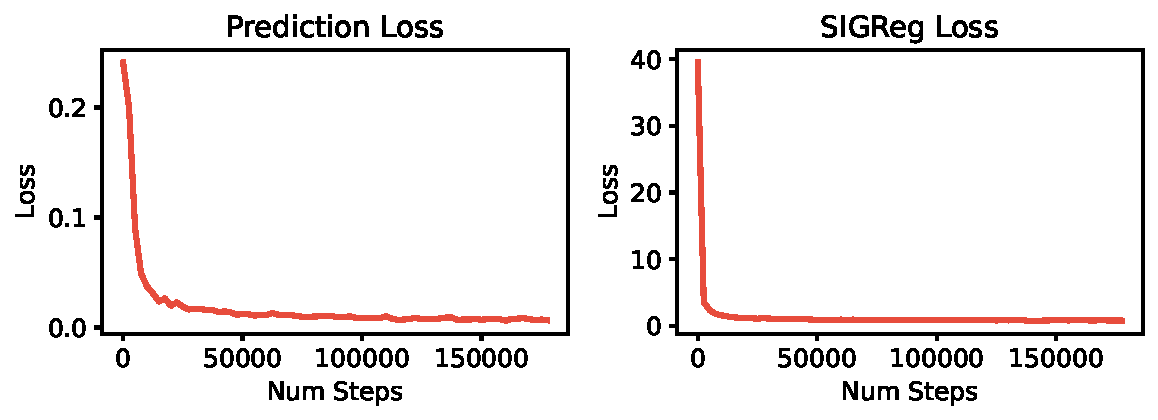
\includegraphics[width=\linewidth]{figs/lewm_pusht_loss.pdf}
    \caption{\textbf{Push-T Training curves for LeWM.}}
    \label{fig:lewm-loss}
\end{figure}

\begin{figure}
    \centering
    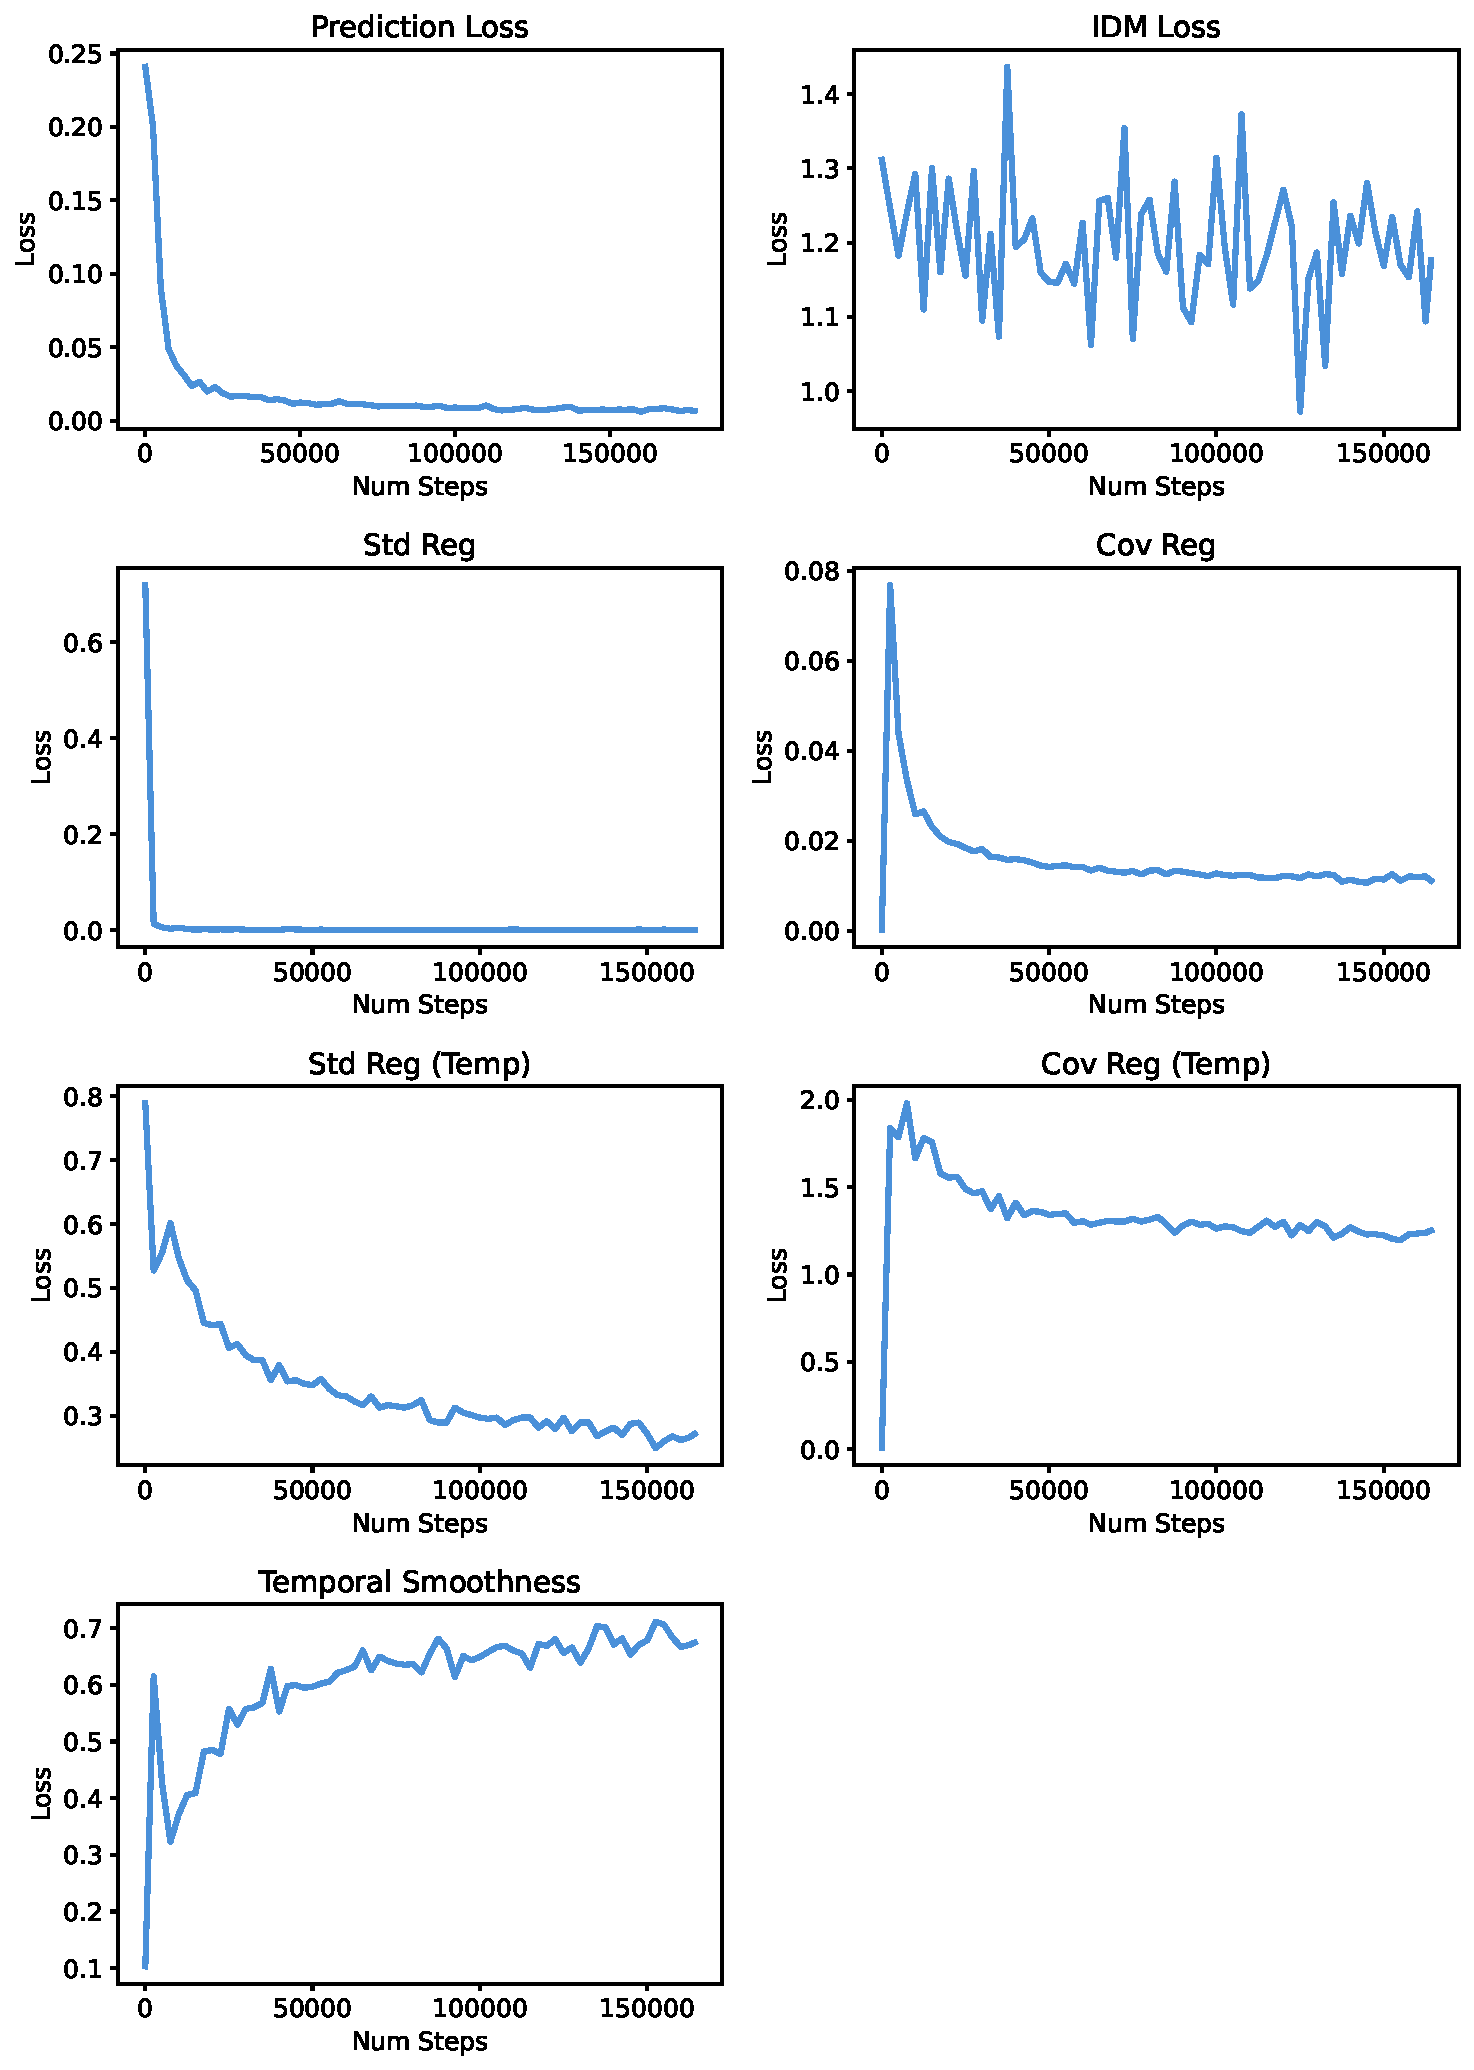
\includegraphics[width=\linewidth]{figs/pldm_pusht_loss.pdf}
    \caption{\textbf{Push-T Training curves for PLDM.}}
    \label{fig:pldm-loss}
\end{figure}
